\documentclass{article}

\usepackage{graphicx}
\usepackage{tikz}
\usepackage{tikzsymbols}
\usetikzlibrary{calc,patterns,shapes.geometric}
\pagestyle{empty}
\usepackage[margin=0pt]{geometry}
\geometry{papersize={14in,12in}}

\def\centerarc[#1](#2)(#3:#4:#5){\draw[#1] ($(#2)+({#5*cos(#3)},{#5*sin(#3)})$) arc (#3:#4:#5);}

\begin{document}
	\begin{figure}
		\centering
		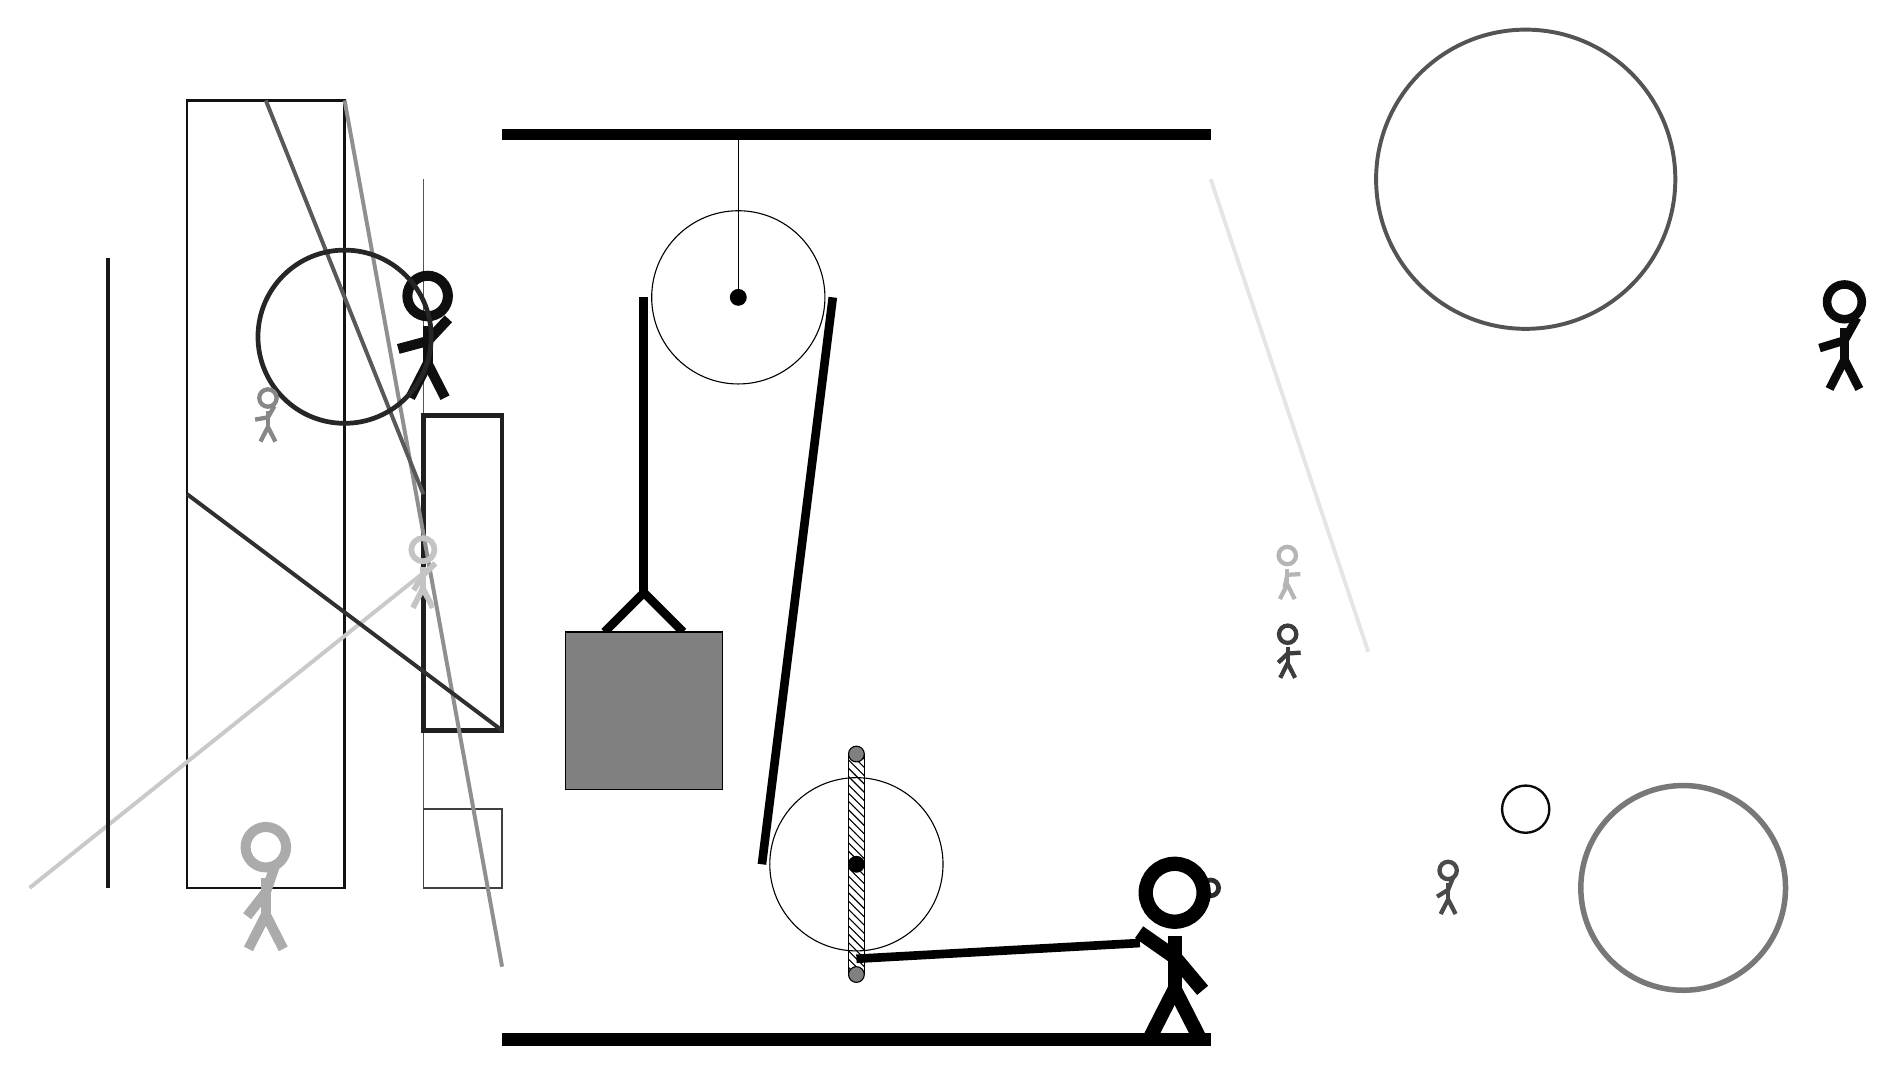
\begin{tikzpicture}
			%%%%% START %%%%%
			
			\draw[fill=black] (-2, 11.5) rectangle (7, 11.625);
			
			\draw (1, 9.5) circle (1.1);
			\draw[fill=black] (1, 9.5) circle (0.1);
			\draw (1, 11.5) -- (1, 9.5);
			
			\draw[fill=white](2.5, 2.3) circle (1.1);
			\draw[fill=black] (2.5, 2.3) circle (0.1);
			\draw[pattern=north west lines, pattern color=black] (2.4, 3.7) rectangle (2.6, 0.9);
			\draw[fill=black!50] (2.5, 3.7) circle (0.1);
			\draw[fill=black!50] (2.5, 0.9) circle (0.1);
			
			\draw[line width=1.1mm] (-0.7, 5.25) -- (-0.2, 5.75) -- (0.3, 5.25);
			\draw[fill=black!50] (-1.2, 5.25) rectangle (0.8, 3.25);
			
			\draw[line width=0.2mm, color=black!67] (-3, 3) rectangle (-3, 11);
			
			\draw[line width=0.3mm, color=black!93] (-4, 2) rectangle (-6, 12);
			\draw[line width=0.6mm, color=black!88] (-3, 4) rectangle (-2, 8);
			\draw[line width=0.2mm, color=black!75] (-3, 3) rectangle (-2, 2);
			\node[line width=0.6mm, color=black!76] at (8, 5) {\Strichmaxerl[3][44][4]};
			\node[line width=0.4mm, color=black!94] at (-3, 9) {\Strichmaxerl[7][15][47]};
			\draw[line width=0.5mm, color=black!44](-2, 1) -- (-4, 12);
			\draw[line width=0.5mm, color=black!21](-3, 6) -- (-8, 2);
			\draw[line width=0.5mm, color=black!65](-3, 7) -- (-5, 12);
			\draw [line width=0.5mm, color=black!67](11, 11) circle (1.9);
			
			\draw [line width=0.6mm, color=black!85](-4, 9) circle (1.1);
			
			\node[line width=0.6mm, color=black!33] at (-5, 2) {\Strichmaxerl[7][52][71]};
			\node[line width=0.3mm, color=black!47] at (-5, 8) {\Strichmaxerl[3][10][60]};
			
			\draw [line width=0.6mm, color=black!83](7, 2) circle (0.1);
			\draw[line width=0.5mm, color=black!91](-7, 10) -- (-7, 2);
			\draw[line width=0.5mm, color=black!81](-2, 4) -- (-6, 7);
			
			\node[line width=0.3mm, color=black!23] at (-3, 6) {\Strichmaxerl[4][58][44]};
			\draw [line width=0.7mm, color=black!53](13, 2) circle (1.3);
			\draw [line width=0.3mm, color=black!96](11, 3) circle (0.3);
			\draw [line width=0.7mm, color=black!61](11, 9) circle (0.0);
			\node[line width=0.3mm, color=black!71] at (10, 2) {\Strichmaxerl[3][32][68]};
			
			\draw[line width=0.5mm, color=black!10](7, 11) -- (9, 5);
			
			\node[line width=0.6mm, color=black!29] at (8, 6) {\Strichmaxerl[3][78][3]};
			\node[line width=0.7mm, color=black!96] at (15, 9) {\Strichmaxerl[6][17][61]};
			
			\draw[line width=1.1mm] (-0.2, 9.5) -- (-0.2, 5.75);
			\centerarc[line width=1.1mm](1, 9.5)(0:180:1.2000000000000002);
			\draw[line width=1.1mm](2.2, 9.5) -- (1.3, 2.3);
			\centerarc[line width=1.1mm](2.5, 2.3)(180:270:1.2000000000000002);
			\draw[line width=1.1mm](2.5, 1.1) -- (6.1, 1.3);
			
			\node at (6.5, 1.2) {\Strichmaxerl[10][-35][-50]};
			
			\draw[fill=black] (-2, 0) rectangle (7, 0.15);
			
			%%%%% END %%%%%
		\end{tikzpicture}
	\end{figure}	
\end{document}